\chapter{Projeto de estudo de Caso}
\label{estudo de caso}

Este capítulo irá apresentar o projeto do estudo de caso que foi realizado no passo planejar estudo de caso, este passo consiste na elaboração de um protocolo para o estudo de caso, na identificação do problema e na definição das questões e objetivos de pesquisa. O método para coleta dos dados e como eles serão analisados também serão expostos neste capítulo.

\section{Definição}

Segundo \cite{yin2001estudo} o estudo de caso é um conjunto de procedimentos pré-especificados para se obter uma investigação empírica que investiga um fenômeno contemporâneo dentro de seu contexto da vida real, especialmente quando os limites entre o fenômeno e o contexto não estão claramente definidos. Uma grande vantagem do estudo de caso é a sua capacidade de lidar com uma ampla variedade de evidências - documentos, artefatos, entrevistas e observações - além do que pode estar disponível no estudo histórico convencional. Além disso, em algumas situações, como na observação participante, pode ocorrer manipulação informal.

Buscando maior entendimento a respeito do estudo de caso proposto, foram criadas algumas perguntas que são fundamentais para o seu entendimento:

\begin{easylist}[itemize]	
	
	& Qual o escopo do estudo de caso?
	& Qual o problema a ser tratado?
	& Qual a questão de pesquisa relacionada a esse problema?
	& Quais são os objetivos a serem alcançados nessa pesquisa?	
	& Como foi a seleção do estudo de caso?
	& Qual é fonte dos dados coletados nessa pesquisa e qual o método de coleta?
	
	\end{easylist}	
	
Com o objetivo da elucidação do escopo do estudo de caso proposto neste trabalho apresentado na Figura \ref{EscopoEstudoCaso},foi apresentado nos capítulos antecedentes, um estudo teórico  relacionado à métricas de software, contratação de serviços de TI em administrações públicas brasileiras e de Data \textit{Warehouse}. Também foi apresentado uma solução para o monitoramento de Métricas de Código-Fonte com suporte de um ambiente de Data \textit{Warehousing}.

\begin{figure}[h!]
\centering
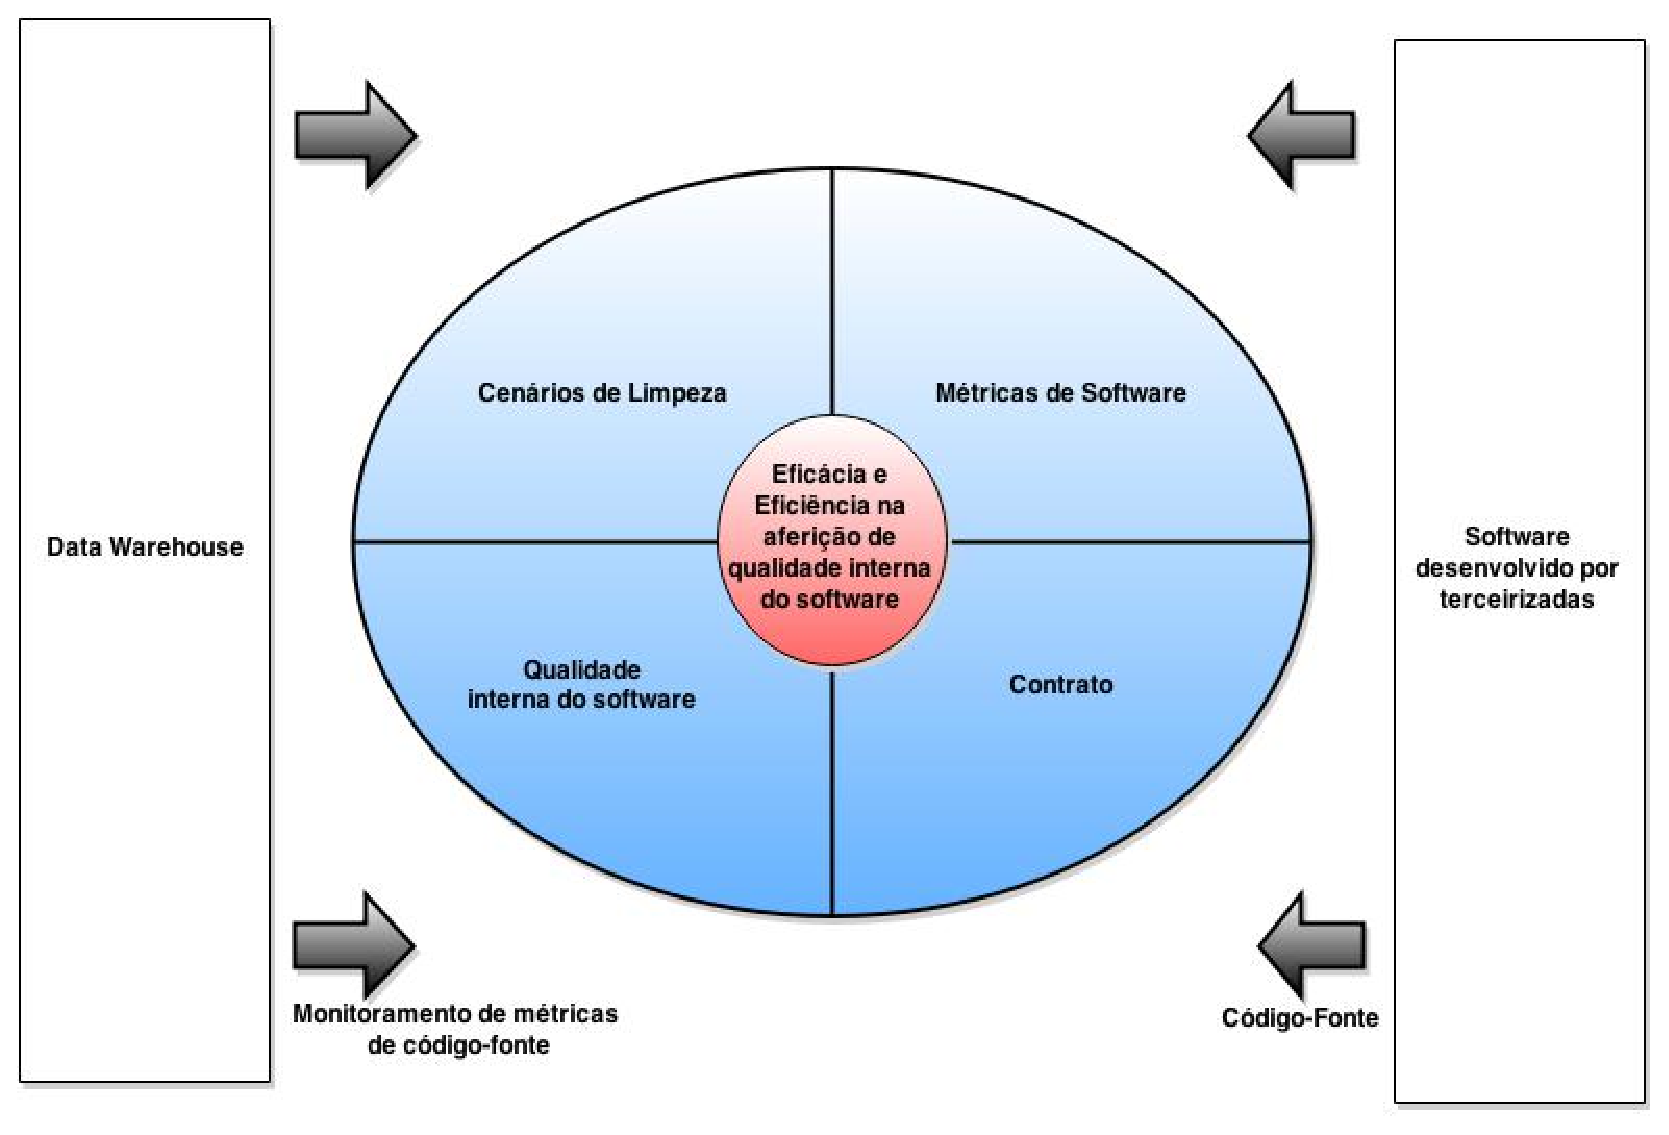
\includegraphics[keepaspectratio=false,scale=0.5]{figuras/figuras_nilton/EscopoEstudoCaso.eps}
\caption{Escopo do Estudo de Caso}
\label{EscopoEstudoCaso}
\end{figure}

Portanto o fundamento da proposta deste trabalho está ligado à análise e coleta de  métricas de código-fonte e de cenários de limpeza de um \textit{software}, desenvolvido por uma empresa terceirizada contratada por um órgão público brasileiro, utilizando uma solução de DW. Onde o foco será será evidenciar a eficácia e a eficiência da proposta por \citeonline{rego_monitoramento_2014} no aferimento de qualidade do software adquirido de uma empresa terceirizada pela equipe responsável do Órgão público e seus demais envolvidos.
	
Para  as demais perguntas serem respondidas, foi estruturado neste trabalho um problema, uma questão de pesquisa, objetivos e questões específicas conforme ilustrado na Figura \ref{EstruturaEstudoCaso}.

\begin{figure}[h!]
\centering
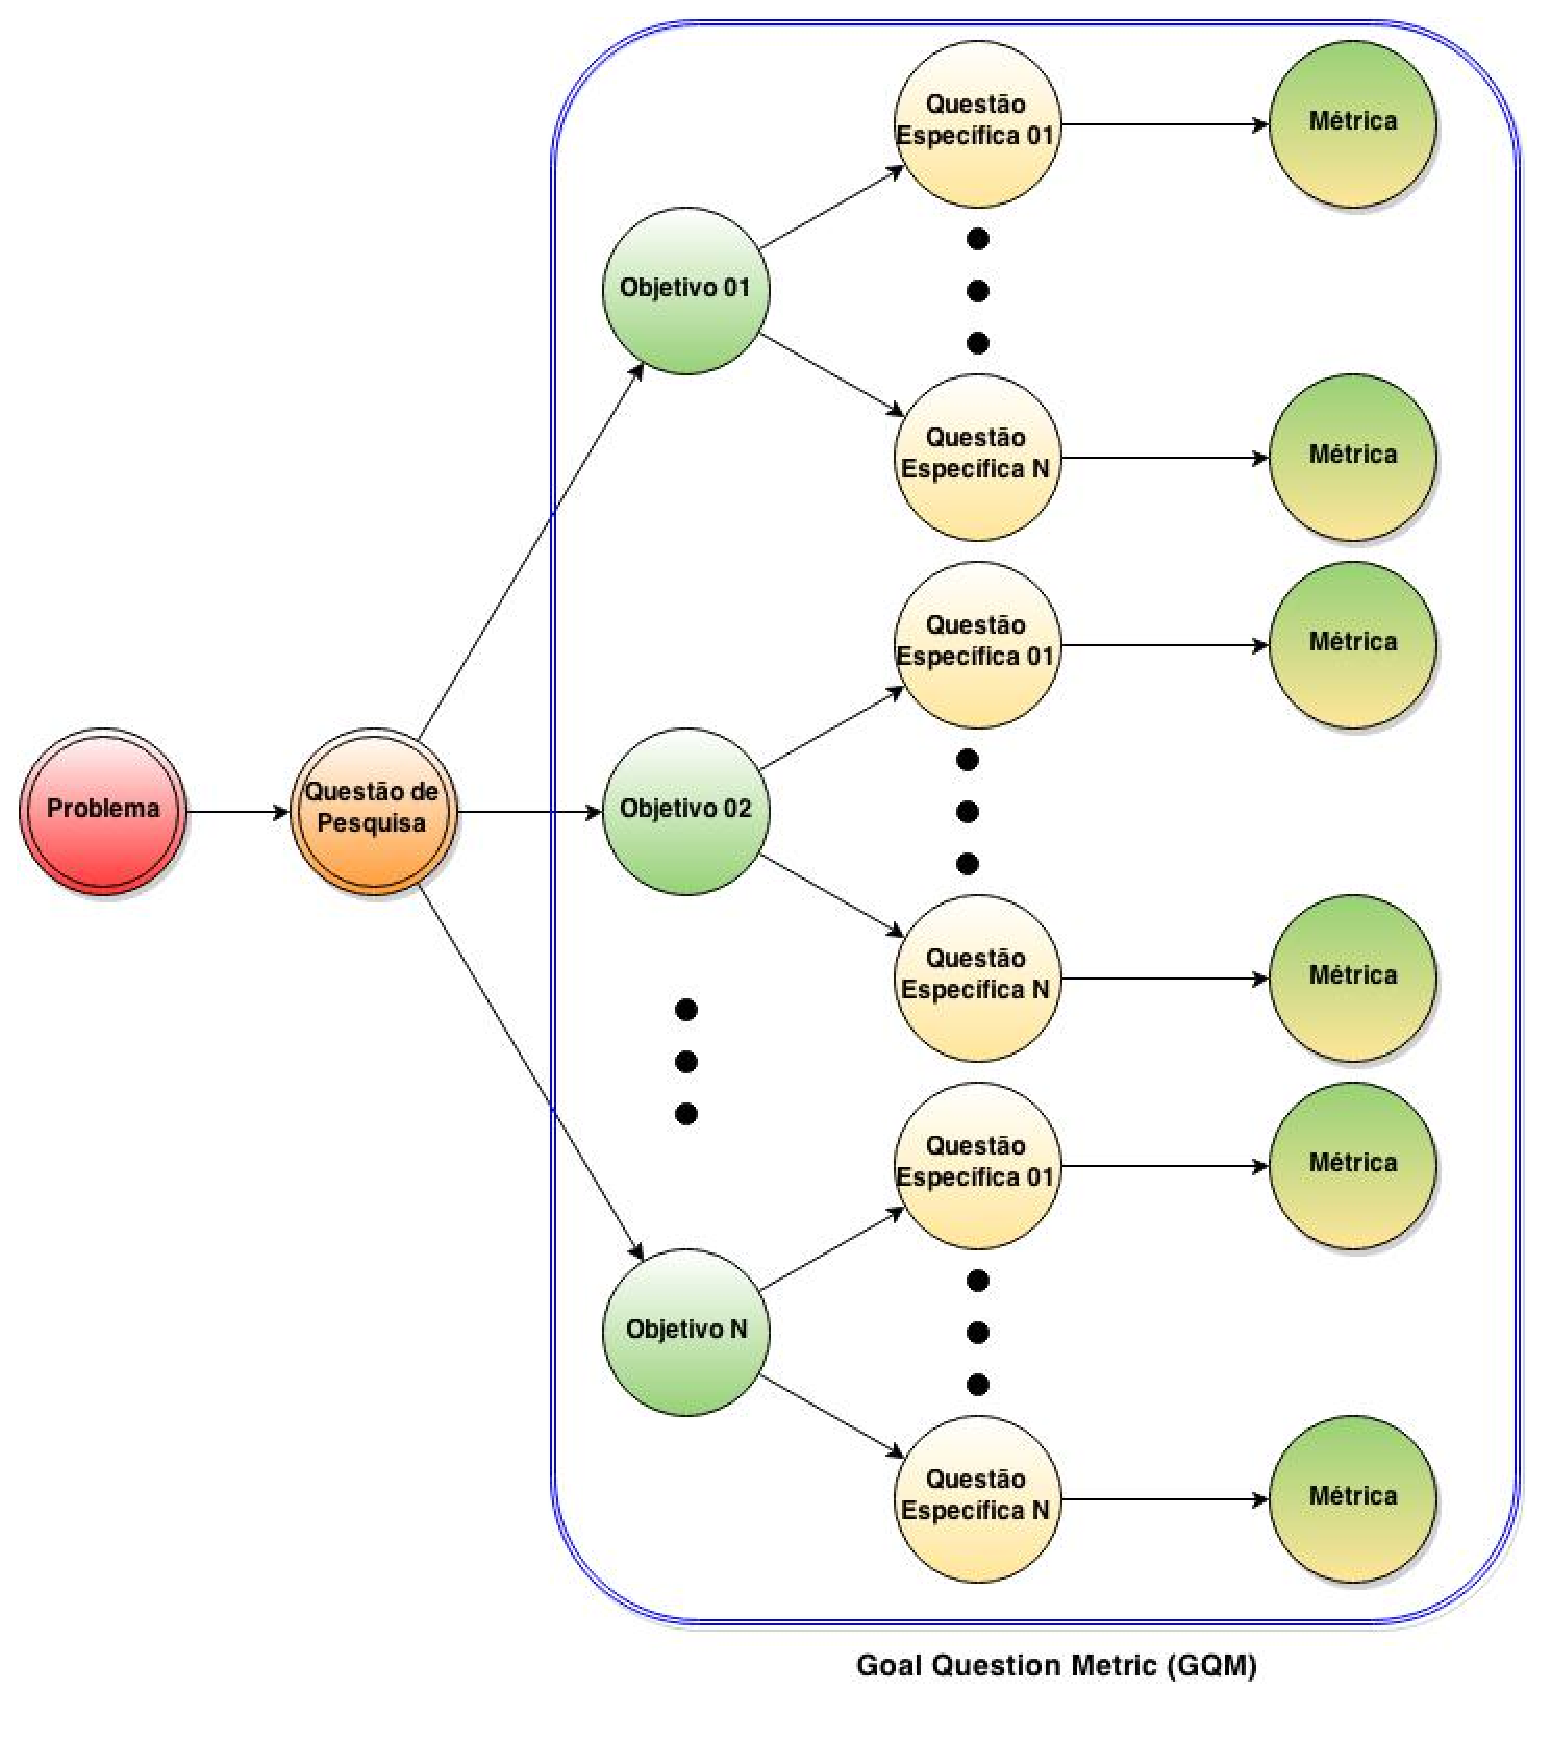
\includegraphics[keepaspectratio=false,scale=0.5]{figuras/figuras_nilton/EstruturaEstudoCaso.eps}
\caption{Estrutura do Estudo de Caso}
\label{EstruturaEstudoCaso}
\end{figure}


\subsection{Problema}

O problema refere-se ao problema de pesquisa identificado na seção "Problema" do capítulo um.

\textbf{A falta de capacidade da administração pública de aferir a qualidade interna dos produtos de software adquiridos e desenvolvidos por empresas contratadas.}

\subsection{Questão de Pesquisa}

A questão de pesquisa refere-se a questão de pesquisa identificada na seção "Questão de Pesquisa" do capítulo um. 

\textbf{O uso de DW para o monitoramento de métricas de código fonte para assistir ao processo de aferição de qualidade interna dos produtos de software desenvolvido por terceirizadas, do ponto de vista da equipe de qualidade no desenvolvimento de software no órgão público, é eficaz e eficiente?}

Para atender a questão de pesquisa foi utilizado o mecanismo \textit{goal-question-metrics}. Segundo \cite{Basili96b} o resultado da aplicação do GQM é a especificação de um sistema de medida destinada a um conjunto especifico de questões e um conjunto de regras para a interpretação dos dados da medição. O GQM é uma estrutura hierárquica que começa com um objetivo que especifica o propósito da medição, objeto a ser medido, questão a ser medida e o ponto de vista de que a medida seja tomada. O objetivo é refinado em várias questões, cada questão é transformada em métrica(objetiva ou subjetiva)\cite{Basili96b}. A estrutura do GQM está a seguir.

\textbf{Objetivo 01:} Avaliar a eficácia e eficiência do uso de \textit{Data Warehouse} para monitoramento de métricas de código fonte.\\


% Questão 01

\textbf{QE01:} Quantas tomadas de decisão foram realizadas pela equipe baseando-se no uso da solução desenvolvida em um <período de tempo>?

\textbf{Fonte:} Registro de observação em campo.

\textbf{Métrica:} Número de decisões tomadas/tempo. \\


% Questão 02

\textbf{QE02: } Quantas tomadas de decisão ao todo foram realizadas pela equipe baseando-se no uso da solução desenvolvida?

\textbf{Fonte:} Registro de observação em campo.

\textbf{Métrica:} Número de decisões tomadas.\\


% Questão 03

\textbf{QE03: } Qual a avaliação da equipe de qualidade quanto a detecção de cenários de limpeza de código?

\textbf{Fonte:} Questionário com equipe de qualidade.

\textbf{Métrica:} muito bom, bom, regular, ruim, muito ruim.\\


% Questão 04

\textbf{QE04: } Com que frequência a equipe de qualidade encontra falhas relacionados à utilização da ferramenta em um determinado intervalo de tempo?

\textbf{Fonte:} Registro de observação em campo.

\textbf{Métrica:} Quantidade de falha / tempo (release, sprint).

\textbf{Interpretação da métrica:} Quanto mais próximo de zero melhor 0=<X\\


% Questão 05

\textbf{QE05: } Qual a quantidade total de falhas encontradas pela equipe de qualidade relacionadas à utilização da ferramenta?

\textbf{Fonte:} Registro de observação em campo (áudio/vídeo).

\textbf{Métrica:} Quantidade de falhas.\\


% Questão 06

\textbf{QE06: } Qual a proporção do uso da ferramenta para tomada de decisões?

\textbf{Fonte:} Questionário com equipe de qualidade.

\textbf{Métrica:} Número de decisões tomadas / número de vezes que a solução foi usada.\\



% Questão 07

\textbf{QE07: } Qual a quantidade de cenários que foram corrigidos após utilização da solução?

\textbf{Fonte:} Código fonte.

\textbf{Métrica:} Números de cenários corrigidos / número de cenários encontrados.\\


% Questão 08

\textbf{QE08: } Qual o nível de satisfação do uso da solução em comparação à solução anterior? 

\textbf{Fonte:} Equipe de qualidade.

\textbf{Métrica:} Muito satisfeito, Satisfeito, Neutro, Insatisfeito, Muito Insatisfeito.\\


% Questão 09

\textbf{QE09: } Qual a taxa de oportunidade de melhoria de código em uma intervalo de tempo (sprint, release)? 

\textbf{Fonte:} Código fonte.

\textbf{Métrica:} Taxa de oportunidade de melhoria de código: $$ T_r =   \frac{{\sum_{i=1}^{n}{Ce_i}}}{\sum_{i=1}^{n}{Cl_i}} $$ $ Ce $ é o total de cenários de limpezas identificados e $ Cl $  é o total de classes em um intervalo de tempo (sprint, release).

\textbf{Interpretação da métrica: } 

\begin{easylist}[itemize]	
	& Número de classes crescente e constante, Número de oportunidade de melhoria estável: Projeto cresceu mais dos 	que o cenários, cenários podem ou não estar sendo tratados.
	& Número de classes crescente e constante, Número de oportunidade de melhoria crescendo: Projeto cresce junto 		com cenários que não são tratados com eficiência ou não são tratados
	& Número de classes crescente ou não, mas constante, número de oportunidade de melhoria diminuindo: Projeto 		cresce e cenários são tratados com eficiência.	
	\end{easylist}	
	

\section{\textit{Background}}

Referente ao contexto deste trabalho, o principal \textit{background} é o trabalho desenvolvido por \citeonline{rego_monitoramento_2014}, no qual utilizaremos sua solução para monitorar as métricas de código-fonte utilizando \textit{Data Warehouse}.
\citeonline{novello_uma_2006} utilizou \textit{Data Warehouse} para monitoramento de métricas no processo de desenvolvimento de software, porém são métricas voltadas para a qualidade do processo de desenvolvimento de software mas são diretamente relacionadas ao código-fonte. Portanto o levantamento bibliográfico realizado, não foram encontrados estudos que utilizassem \textit{Data Warehouse} para aferir qualidade interna do \textit{software }aplicando coleta de métricas de código-fonte e geração de cenários de limpeza assim como foi feito por \citeonline{rego_monitoramento_2014}.

%\section{Seleção}

%Os dados foram coletados na CAIXA porque ?????????????????????????????????

\section{Fonte dos dados coletados e método de coleta}

Os dados deste estudo de caso,serão coletados através de registros de observações em campo, questionários, entrevistas e resultados gerados pela própria solução utilizando o código-fonte de um ou mais sistemas desenvolvidos por empresas contratadas pelo órgão público.

Os registros oriundos de observações em campo são gerados a partir da equipe responsável pela tomada de decisões de qualidade e são coletados durante as visitas realizadas no órgão público. Nessas visitas, a solução proposta é utilizada e qualquer atitude relacionada ao seu uso pela equipe é registrada e será do ponto de vista qualitativo e quantitativo.

A adoção de questionários também foi utilizada tanto para dados qualitativos quanto para dados quantitativos á respeito da solução de DW vista pela equipe responsável e os demais envolvidos na qualidade de \textit{software} no órgão público, no que diz respeito à tomadas de decisões, detecção de cenários de limpeza de código, falhas relacionados à utilização da ferramenta adotada na solução de DW, ao nível de satisfação no uso da solução e as taxas de oportunidades de melhoria de código. 

Os gráficos e resultados gerados pela solução de DW, serão coletados a medida que a solução for utilizada pela equipe de qualidade ao longo das releases dos projetos adotados.

\section{Ameaças a validade do estudo de caso}

\citeonline{yin2001estudo} descreve como principais ameaças relacionadas à validade do estudo de caso as ameaças relacionadas à validade do constructo, à validade interna, à validade externa e à confiabilidade. As quatro ameaças definidas por ele, bem como a forma usada nesse trabalho para preveni-las, são descritas da seguinte maneira: 

\begin{easylist}[itemize]	

& \textbf{Validade do Constructo: } A validade de construção está presente na fase de coleta de dados, quando deve ser evidenciado as múltiplas fontes de evidência e a coleta de um conjunto de métricas para que se possa saber exatamente o que medir e quais dados são relevantes para o estudo, de forma a responder as questões de pesquisa \cite{yin2001estudo}. Buscou-se garantir a validade de construção ao definir objetivos com evidências diferentes. Estas, por sua vez, estão diretamente relacionadas com os objetivos do estudo de caso e os objetivos do trabalho. 

& \textbf{Validade interna: } Para \citeonline{yin2001estudo} o uso de várias fontes de dados e métodos de coleta permite a triangulação, uma técnica para confirmar se os resultados de diversas fontes e de diversos métodos convergem. Dessa forma é possível aumentar a validade interna do estudo e aumentar a força das conclusões.
A triangulação de dados se deu pelo resultado da solução de \textit{Data Warehouse} que utiliza o código-fonte (explicada no capítulo \ref{chap:arquitetura} ), pela análise de questionários e pelos dados coletados através de entrevistas.

& \textbf{Validade externa: } Por este ser um caso único, a generalização do estudo de caso se dá de maneira pobre \cite{yin2001estudo}. Assim é necessária a utilização do estudo em múltiplos casos para que se comprove a generalidade dos resultados. Como este trabalho é o primeiro a verificar a eficácia e eficiência da solução para o estudo de caso no órgão, não há como correlacionar os resultados obtidos a nenhum outro estudo.

& \textbf{Confiabilidade: } Com relação a confiabilidade, \citeonline{yin2001estudo} associa à repetibilidade, desde que seja usada a mesma fonte de dados. Nesse trabalho o protocolo de estudo de caso apresentado nessa seção garantem a repetibilidade desse trabalho e consequentemente a validade relacionada à confiabilidade.

\end{easylist}	


\section{Processo de análise dos dados}

Análise dos dados coletados durante o estudo de caso a ser realizado no TCU? será feita através de 4 etapas:

\begin{easylist}[itemize]	
	
	& \textbf{Categorização: } Organização dos dados em duas categorias - qualitativos e quantitativos. Os dados qualitativos referem-se aos questionários realizados. Os dados quantitativos, por sua vez, referem-se aos valores numéricos da solução de DW para monitoramento de métricas. 
	& \textbf{Exibição: } Consiste na organização dos dados coletados para serem exibidos através de gráficos, tabelas e texto para poderem ser analisados. 
	& \textbf{Verificação: } Atestar padrões, tendências e aspectos específicos dos significados dos dados. Procurando assim gerar uma discussão e interpretação de cada dado exibido.
	& \textbf{Conclusão: } Agrupamento dos resultados mais relevantes das discussões e interpretações dos dados anteriormente apresentados.
	
	\end{easylist}	


\section{Considerações finais do capítulo}

Esse capítulo teve como objetivo apresentar o protocolo de estudo de caso que será adotado na continuação deste trabalho. No trabalho de conclusão de curso dois serão detalhados o órgão público onde será aplicado o projeto de estudo de caso desenhado neste trabalho, os termos do contrato do órgão e a empresa contratada referentes a qualidade de \textit{software} e serão apresentados os resultados obtidos para as questões específicas apresentadas neste capítulo assim como a interpretação dos mesmos possibilitando responder a questão de pesquisa abordada.  